\subsection*{Node.js chat application}
We havn't been able to break our chat application.
We're not accepting user input, via query arguments and hence the only input method is the chat-username and chat-messages.

Username and message are transfered as JSON, which removes the possibility of directly sending functions to break the server.
We've tried several approaches to break the server code, but as it interacts minimally with the send json, there's not a lot of room for error.
In essence it just forwards one users JSON message to other users.  

Back at the users end, we may now be recieving script tags and whatnot from other users.
Once we recieve a message, we do nothing with it, but to append it to the textarea's value.
This property is resposible for escaping all attempts at tags, be it scripts or html.

Several of our attempts can be seen on the picture below;

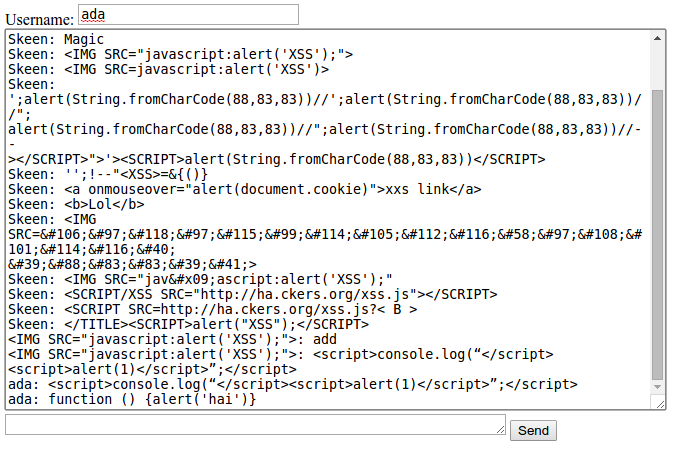
\includegraphics[width=\textwidth]{hoax.png}
We invite the reviewer to attempt to break the system.

The system does have a somewhat staggering weakness to phishing, as there's no mechanism in place to differentiate between users impersonating one another.

Say Alice is chatting with Bob, and Carol is passivly following the chat.
Carol decides to mess with Alice, so she changes her username to Bob, and sends a message, as if she was him.
Bob will be able to see this message no problem, but before he gets to warn Alice that the message wasn't send by him, the damage may already have been invoked.

\subsubsection*{Extensions}
A logical extension to avoid the above weakness to phishing would be the introduction of user accounts.
This would however introduce all of the XSS weaknesses commonly known to roam in those waters.

And alternative extension which could be troublesome, is to display messages in a different manner, say though the use of lists, and via the \verb|.innerHTML| property.
This way we'll have to handle escaping dangerous tags ourselves, which can be error-prone.
An argument for doing this, would be to allow for some limited html markup within the messages.

\subsection*{Dart Picture Browser}
We've been unable to get our client for the Dart Picture Browser to run.
And henceforth unable to test for weaknesses in it's implementation.
